% !TEX encoding = UTF-8
% !TEX TS-program = pdflatex
% !TEX root = ../tesi.tex

%**************************************************************
\chapter{L'azienda}
\label{cap:azienda}
%**************************************************************
\section{Introduzione}
Wavelop è un’azienda giovane e innovativa, con sede operativa a Treviso e sede legale a Venezia, che si occupa dello \
sviluppo di applicazioni web e \emph{mobile} per \emph{startup} e imprese. L’ambiente è informale e dinamico, con un focus \
alla flessibilità e al lavoro da remoto. \\

L’azienda riesce a soddisfare le richieste dei clienti grazie all’utilizzo della metodologia Agile Scrum ed \
alla creazione di \emph{design user-centered}, realizzando \emph{\gls{mock-up}} e prototipi per ottenere i risultati più adatti. \
Vengono, inoltre, utilizzate le migliori tecnologie in base al progetto richiesto.

%**************************************************************
\section{Tecnologie utilizzate}

\subsection{\emph{\Gls{backend}}}

\begin{itemize}
  \item \textbf{\emph{TypeScript}}: linguaggio basato su JavaScript, sviluppato da Microsoft, al quale viene aggiunta \
  la definizione statica dei tipi. Tutto ciò porta ad un rischio minore di \emph{bugs};
  \item \textbf{\emph{Node.js}}: è un sistema \emph{runtime} per JavaScript orientato agli eventi asincroni, è progettato \
  per realizzare applicazioni di rete scalabili;
  \item \textbf{\emph{MongoDB}}: è un \emph{database} NoSQL \emph{document-oriented}, permette di sviluppare applicazioni \
  flessibili e che possono scalare facilmente;
  \item \textbf{Servizi \emph{\acrfull{aws}}}: sono i servizi \emph{cloud} forniti da Amazon che comprendono: \
  \emph{cloud-computing}, archiviazione, \emph{Machine-Learning} e \emph{Internet of Things}. L'azienda utilizza \
  principalmente: 
  \begin{itemize}
    \item AWS Lambda: computazione \emph{serverless};
    \item AWS DynamoDB: \emph{database} NoSQL;
    \item AWS API Gateway: creazione di \acrshort{api}.
  \end{itemize}
\end{itemize}

\subsection{\emph{\Gls{frontend}}}

\begin{itemize}
  \item \textbf{\emph{React}}: è una libreria \emph{\gls{open-source}} JavaScript per realizzare interfacce utente. Sfrutta \
  il principio dello sviluppo per componenti e aggiorna solo i componenti che dipendono dai dati che hanno subito una \
  variazione;
  \item \textbf{\emph{Vue}}: è un \emph{framework} JavaScript \emph{open-source}, orientato al \emph{design pattern} \
  \acrshort{mvvm}, che permette la realizzazione di interfacce utente e \emph{Single Page Application};
  \item \textbf{\emph{Angular}}: è un \emph{framework open-source} basato su TypeScript sviluppato da Google che permette \
  di realizzare applicazioni universali per \emph{desktop}, \emph{mobile} e \emph{tablet}.
\end{itemize}

%**************************************************************
\section{Processi aziendali}

\subsection{Metodologia Agile}
La metodologia Agile è un approccio iterativo al \emph{project management} che consente ai \emph{team} di sviluppo \
di consegnare al cliente il prodotto più rapidamente. In particolare, con lo sviluppo Agile, il \emph{team} si presta a \
lavorare su piccoli incrementi utilizzabili. Ci sono molteplici metodologie che fanno riferimento al \emph{"Agile Manifesto"}, la più diffusa, e utilizzata \
dall'azienda, è lo \emph{Scrum}.

\subsection{\emph{Scrum}}
Lo \emph{Scrum} è un \emph{framework} che incoraggia i membri del \emph{team} a lavorare insieme. È basato sul principio dell'apprendimento continuo e sull'adattamento \
a situazioni che cambiano continuamente, mediante ri-prioritizzazione dei processi e brevi cicli di rilascio, chiamati \textbf{Sprint}, che permettono al \emph{team} di \
imparare e migliorare. Prima di illustrare come lo \emph{Scrum} venga applicato in Wavelop, è bene introdurre i tre artefatti che sono in continuo aggiornamento durante il progetto:

\begin{itemize}
  \item \textbf{\emph{Product Backlog}}: è la lista dei \emph{tasks} che devono essere svolti e viene mantenuta dal \emph{Product Owner}. La lista contiene \emph{features}, \
  requisiti, miglioramenti e correzioni che fungeranno da \emph{input} allo \emph{Sprint Backlog}. I \emph{tasks} presenti nella lista sono costantemente revisionati, mantenuti \
  e, inoltre, possono subire un cambiamento di priorità; 
  \item \textbf{\emph{Sprint Backlog}}: è la lista dei \emph{tasks} selezionati durante l'incontro di pianificazione dello \emph{sprint}, dal \emph{team} di sviluppo, per lo \
  svolgimento nello \emph{sprint cycle} corrente. Lo \emph{sprint backlog} può essere flessibile durante lo \emph{sprint}, ma lo \emph{sprint goal} da raggiungere non deve \
  essere compromesso.
  \item \textbf{Incremento} (o \emph{Sprint Goal}): è il prodotto usabile realizzato durante lo \emph{sprint}. Solitamente viene effettuata una dimostrazione al cliente, \
  attraverso una demo, per mostrare il prodotto realizzato durante lo \emph{sprint} e per ottenere \emph{feedbacks} sul lavoro svolto.
\end{itemize}

Prima inizare uno \emph{sprint}, in Wavelop, il \emph{team} si riusnisce per definire l'obiettivo dello \emph{sprint} che si andrà a svolgere, inoltre vengono selezionate \
dal \emph{product backlog} la \emph{user stories} che dovranno essere implementate durante lo \emph{sprint}: questa attività prende il nome di \emph{Sprint Planning} e, una volta \
terminato, inizia lo \emph{sprint} vero e proprio. In azienda lo \emph{sprint} dura due settimane, durante le quali il \emph{team} implementa le \emph{user stories} presenti \
nello \emph{sprint backlog}. Durante lo \emph{sprint}, ogni mattina prima di iniziare la giornata lavorativa, viene svolto lo \emph{stand up metting}: una brave riunione informale \
tra i membri del \emph{team}, durante la quale ci si allinea sul lavoro svolto e pianifica il lavoro della giornata. In Wavelop ogni componente del \emph{team} deve rispondere alle \
seguenti domande: "Cosa ho fatto ieri?", "Cosa farò oggi?", "Ho avuto qualche problema?". Al termine di ogni \emph{sprint}, si svolge una riunione formale tra il \emph{team} e gli \
\emph{\glspl{stakeholder}} per mostrare il lavoro svolto e per ottenere dei \emph{feedbacks} (\emph{Sprint Review}). Successivamente il \emph{team} svolge un'altra riunione per discutere su cosa migliorare \
nel prossimo \emph{sprint} e su cosa ha funzionato nello \emph{sprint} appena concluso (\emph{Sprint Retrospective}). 

\vspace{20pt}
  \begin{figure}[!ht]
    \begin{center}
      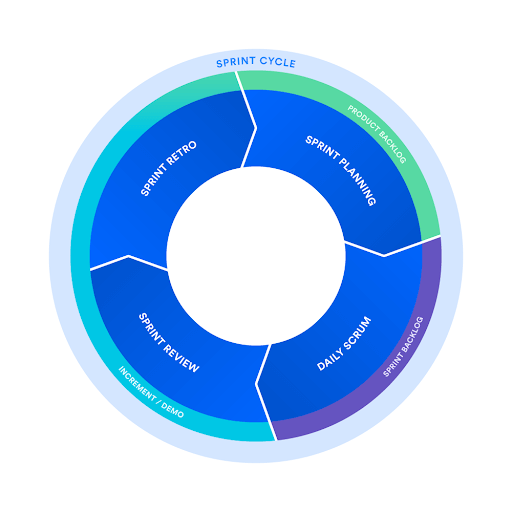
\includegraphics[height=12cm]{sprint-cycle}
      \caption{Ciclo di uno Sprint}
      \textbf{Fonte:} \href{https://www.atlassian.com}{atlassian.com}
    \end{center}
  \end{figure}
\vspace{20pt} 

%**************************************************************
\section{Strumenti a supporto dei processi}

\subsection{Git \& Gitflow Workflow}
\emph{Git} è un \emph{Distributed Version Control System}, \emph{open-source} e gratuito, progettato per gestire progetti di grandi e piccole dimensioni con efficienza. \
Per facilitare la gestione della sviluppo in parallelo e prevenire l'avvento di conflitti, l'azienda ha deciso di utilizzare il modello \emph{Gitflow Workflow}. \
Ogni progetto è costituito da cinque tipi di \emph{branch} diversi: \textbf{\emph{main}}, \textbf{\emph{develop}}, \textbf{\emph{release}}, \textbf{\emph{hotfix}} e \
\textbf{\emph{feature}}. I \emph{branches} di base e che saranno sempre presenti nel ciclo di vita del progetto sono:
\begin{itemize}
  \item \emph{main} nel quale si trova lo storico delle versioni rilasciate in produzione dall'azienda;
  \item \emph{develop} nel quale troviamo lo storico completo del progetto. 
\end{itemize}  

I seguenti tipi di \emph{branch}, a differenza dei precedenti, hanno vita limitata: \
\begin{itemize}
  \item i \emph{branch} di tipo \emph{feature} sono adibiti allo sviluppo di nuove funzionalità, al termine del quale viene incorporato nel \emph{branch develop}; 
  \item i \emph{branch} di tipo \emph{release} vengono utilizzati per cominciare un nuovo ciclo di rilascio per una nuova version, al termine del quale viene incorporato nel \
  \emph{branch main}; 
  \item i \emph{branch} di tipo \emph{hotfix} sono adibiti alla correzione di piccoli \emph{bug} in produzione, una volta risolto il problema viene incorporato nel \emph{branch main}.
\end{itemize}

\vspace{20pt}
  \begin{figure}[!ht]
    \begin{center}
      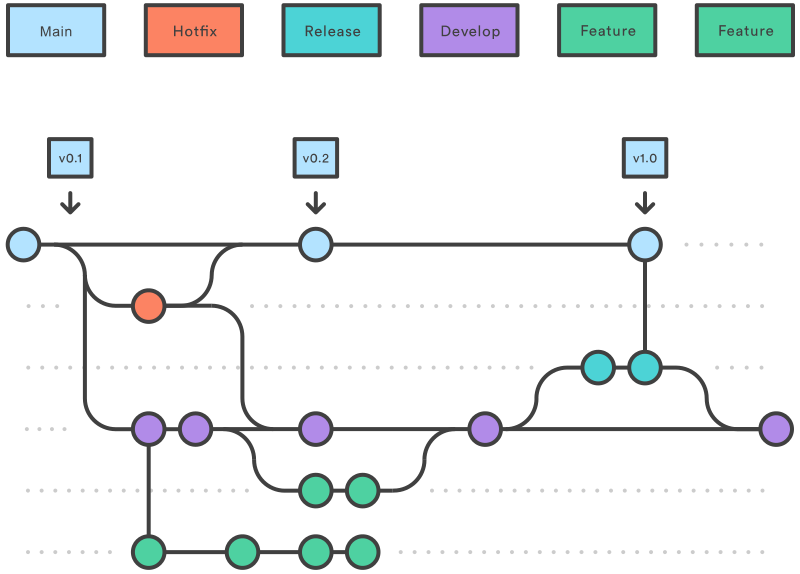
\includegraphics[height=8cm, width=12cm]{gitflow-workflow}
      \caption{Gitflow Workflow}
      \textbf{Fonte:} \href{https://www.atlassian.com}{atlassian.com}
    \end{center}
  \end{figure}
\vspace{20pt} 

\subsection{GitLab}
GitLab, a differenza di git, è una piattaforma di \emph{hosting} per \emph{git repositories}; inoltre offre diversi servizi \
per la gestione del progetto, quali:

\begin{itemize}
  \item \emph{Issue Tracking System};
  \item \emph{Project Board}
\end{itemize}

\subsubsection{\emph{Google Workspace}}
\emph{Google Workspace} è un insieme di strumenti di collaborazione e produttività sviluppato da Google. \
I servizi utilizzati maggiormente dall'azienda sono:

\begin{itemize}
  \item \emph{Gmail} per le comunicazioni formali;
  \item \emph{Calendar} per la gestione degli impegni aziendali;
  \item \emph{Drive} per la memorizzazione di file nel \emph{cloud};
  \item \emph{Meet} per le riunioni con i clienti;
  \item \emph{Google Docs Suite} per la creazione di documenti e presentazioni.
\end{itemize}

%**************************************************************
\section{Rapporto con l'innovazione}
L'azienda è sempre aggiornata sulle nuove tecnologie partecipando ad incontri tecnologici con relatori di spicco: \emph{Google} e \emph{Amazon}, \
per citarne alcuni; in generale, è molto propensa all'innovazione accettando la presa in carico di progetti innovativi che sfruttano \
i moderni \emph{smart speakers}, l'architettura \emph{Serverless} o nell'ambito dell'\acrfull{iot}.